%% LyX 2.3.6.1 created this file.  For more info, see http://www.lyx.org/.
%% Do not edit unless you really know what you are doing.
\documentclass[english]{article}
\usepackage[T1]{fontenc}
\usepackage[latin9]{inputenc}
\usepackage{amsmath}
\usepackage{cancel}
\usepackage{graphicx}
\usepackage{babel}
\begin{document}

\part{definition}

The polarized GPD is defined as
\[
\tilde{F_{q}}=\frac{1}{2P^{+}}[\tilde{H^{q}}(x,\xi,t)\bar{u}(p_{2})\gamma^{+}\gamma_{5}u(p_{1})+\tilde{E^{q}}(x,\xi,t)\bar{u}(p_{2})\frac{\gamma_{5}q^{+}}{2M}u(p_{1})]
\]

Thus the definition of splitting function is 
\[
\bar{u}(p_{2})\Gamma^{+}u(p_{1})=\bar{u}(p_{2})[\gamma^{+}\gamma_{5}\tilde{f}(y,t)+\frac{\gamma_{5}q^{+}}{2M}\tilde{g}(y,t)]u(p_{1})
\]


\part{projection}

For polarized GPD, we want to include the spin of particles, so in
zero skewness case we define this trace term to get the $\tilde{f}$
\begin{align*}
A & =\bar{u}(p_{2})\Gamma^{+}u(p_{1})\bar{u}(p_{1})\gamma^{+}\gamma_{5}u(p_{2})\\
 & =\textrm{Tr}[\Gamma^{+}(\cancel{p_{1}}+m)\frac{1+\gamma_{5}\cancel{s_{1}}}{2}\gamma^{+}\gamma_{5}(\cancel{p_{2}}+m)\frac{1+\gamma_{5}\cancel{s_{2}}}{2}]
\end{align*}

where $s$ is operator of spin which is defined as
\[
s^{\mu}=(\frac{\overrightarrow{p}.\overrightarrow{\lambda}}{m},\overrightarrow{\lambda}+\frac{\overrightarrow{p}(\overrightarrow{p}.\overrightarrow{\lambda})}{m(m+p_{0})})
\]
and we chose $\overrightarrow{\lambda}=(0,0,1)$ in rest frame.

In nonzero skewness case, firstly I follow the equation above and
we have 
\begin{align*}
A & =\bar{u}(p_{2})\Gamma^{+}u(p_{1})\bar{u}(p_{1})\gamma^{+}\gamma_{5}u(p_{2})\\
 & =\textrm{Tr}[\Gamma^{+}(\cancel{p_{1}}+M)\frac{1+\gamma_{5}\cancel{s_{1}}}{2}\gamma^{+}\gamma_{5}(\cancel{p_{2}}+M)\frac{1+\gamma_{5}\cancel{s_{2}}}{2}]\\
B & =\bar{u}(p_{2})\Gamma^{+}u(p_{1})\bar{u}(p_{1})\frac{\gamma_{5}q^{+}}{2M}u(p_{2})\\
 & =\textrm{Tr}[\Gamma^{+}(\cancel{p_{1}}+M)\frac{1+\gamma_{5}\cancel{s_{1}}}{2}\frac{\gamma_{5}q^{+}}{2M}(\cancel{p_{2}}+M)\frac{1+\gamma_{5}\cancel{s_{2}}}{2}]
\end{align*}

However, replace $\Gamma^{+}$ with $\tilde{f}\ \tilde{g}$
\begin{align*}
A & =\bar{u}(p_{2})\left(\gamma^{+}\gamma_{5}\tilde{f}(y,t)+\frac{\gamma_{5}q^{+}}{2M}\tilde{g}(y,t)\right)u(p_{1})\bar{u}(p_{1})\gamma^{+}\gamma_{5}u(p_{2})\\
 & =\bar{u}(p_{2})\gamma^{+}\gamma_{5}\tilde{f}(y,t)u(p_{1})\bar{u}(p_{1})\gamma^{+}\gamma_{5}u(p_{2})\\
 & +\bar{u}(p_{2})\frac{\gamma_{5}q^{+}}{2M}\tilde{g}(y,t)u(p_{1})\bar{u}(p_{1})\gamma^{+}\gamma_{5}u(p_{2})\\
B & =\bar{u}(p_{2})\left(\gamma^{+}\gamma_{5}\tilde{f}(y,t)+\frac{\gamma_{5}q^{+}}{2M}\tilde{g}(y,t)\right)u(p_{1})\bar{u}(p_{1})\frac{\gamma_{5}q^{+}}{2M}u(p_{2})\\
 & =\bar{u}(p_{2})\gamma^{+}\gamma_{5}\tilde{f}(y,t)u(p_{1})\bar{u}(p_{1})\frac{\gamma_{5}q^{+}}{2M}u(p_{2})\\
 & +\bar{u}(p_{2})\frac{\gamma_{5}q^{+}}{2M}\tilde{g}(y,t)u(p_{1})\bar{u}(p_{1})\frac{\gamma_{5}q^{+}}{2M}u(p_{2})
\end{align*}

If we express the equation above in this way
\begin{align*}
A & =a_{1}*f+a_{2}*g\\
B & =b_{1}*f+b_{2}*g
\end{align*}

then the $\tilde{f}\ \tilde{g}$ is 
\begin{align*}
f & =\frac{a_{2}B-b_{2}A}{a_{2}b_{1}-a_{1}b_{2}}\\
g & =\frac{b_{1}A-a_{1}B}{a_{2}b_{1}-a_{1}b_{2}}
\end{align*}

The coefficient $a_{i}\ b_{i}$ is, with the spinor 
\begin{align*}
a_{2}b_{1}-a_{1}b_{2} & =\bar{u}(p_{2})\frac{\gamma_{5}q^{+}}{2m}u(p_{1})\bar{u}(p_{1})\gamma^{+}\gamma_{5}u(p_{2})*\bar{u}(p_{2})\gamma^{+}\gamma_{5}u(p_{1})\bar{u}(p_{1})\frac{\gamma_{5}q^{+}}{2M}u(p_{2})\\
 & -\bar{u}(p_{2})\gamma^{+}\gamma_{5}u(p_{1})\bar{u}(p_{1})\gamma^{+}\gamma_{5}u(p_{2})*\bar{u}(p_{2})\frac{\gamma_{5}q^{+}}{2m}u(p_{1})\bar{u}(p_{1})\frac{\gamma_{5}q^{+}}{2M}u(p_{2})\\
 & =0
\end{align*}

notice the terms like $\bar{u}(p_{2})\frac{\gamma_{5}q^{+}}{2m}u(p_{1})$
is a number and is commutative. And we always have the result $a_{2}b_{1}-a_{1}b_{2}=0$
no matter the $\gamma$ matrix we chose in $AB$.

If we use this definition 
\begin{align*}
A & =\underset{s_{1}}{\Sigma}\bar{u}^{s_{2}}(p_{2})\Gamma^{+}u^{s_{1}}(p_{1})\bar{u}^{s_{1}}(p_{1})\gamma^{+}\gamma_{5}u^{s_{2}}(p_{2})\\
 & =\textrm{Tr}[\Gamma^{+}(\cancel{p_{1}}+M)\gamma^{+}\gamma_{5}(\cancel{p_{2}}+M)\frac{1+\gamma_{5}\cancel{s_{2}}}{2}]\\
B & =\underset{s_{1}}{\Sigma}\bar{u}^{s_{2}}(p_{2})\Gamma^{+}u^{s_{1}}(p_{1})\bar{u}^{s_{1}}(p_{1})\frac{\gamma_{5}q^{+}}{2M}u^{s_{2}}(p_{2})\\
 & =\textrm{Tr}[\Gamma^{+}(\cancel{p_{1}}+M)\frac{\gamma_{5}q^{+}}{2M}(\cancel{p_{2}}+M)\frac{1+\gamma_{5}\cancel{s_{2}}}{2}]
\end{align*}

the A B are not degenerate and we can get $\tilde{f}\ \tilde{g}$

\section{rainbow diagram }

\[
\Gamma^{+}=\int d^{4}k\cancel{k}\gamma_{5}\widetilde{F}^{2}(k)\frac{1}{D_{\phi}(k)}\frac{\cancel{p'}-\cancel{k}+m_{N}}{D_{B}(p'-k)}\gamma^{+}\gamma_{5}\frac{\cancel{p}-\cancel{k}+m_{N}}{D_{B}(p-k)}\cancel{k}\gamma_{5}\delta(y-\frac{k^{+}}{P^{+}})
\]

Like the unpolarized case, we have $\delta$ term which is also calculated
in similar way like unpolarized GPD. And follow the new definition
of projection, we can get a $\xi$ independent result of $\tilde{f}\ \tilde{g},$where
I omit some coefficient 
\begin{align*}
\int_{0}^{1-\xi}dy\tilde{f_{1}}(y)+\int_{1-\xi}^{1+\xi}dy\tilde{f_{2}}(y)+\tilde{f_{\delta}} & =1.79\\
\int_{0}^{1-\xi}dy\tilde{g_{1}}(y)+\int_{1-\xi}^{1+\xi}dy\tilde{g_{2}}(y)+\tilde{g_{\delta}} & =2.43
\end{align*}

In $q^{+}=0$ case, we can check the two definition of projection
which is 
\begin{align*}
A & =\bar{u}(p_{2})\Gamma^{+}u(p_{1})\bar{u}(p_{1})\gamma^{+}\gamma_{5}u(p_{2})\\
 & =\bar{u}(p_{2})\gamma^{+}\gamma_{5}\tilde{f}(y,t)u(p_{1})\bar{u}(p_{1})\gamma^{+}\gamma_{5}u(p_{2})\\
 & =\textrm{Tr}[\gamma^{+}\gamma_{5}(\cancel{p_{1}}+m)\frac{1+\gamma_{5}\cancel{s_{1}}}{2}\gamma^{+}\gamma_{5}(\cancel{p_{2}}+m)\frac{1+\gamma_{5}\cancel{s_{2}}}{2}]\tilde{f}(y,t)
\end{align*}

and 
\begin{align*}
A' & =\underset{s_{1}}{\Sigma}\bar{u}^{s_{2}}(p_{2})\Gamma^{+}u^{s_{1}}(p_{1})\bar{u}^{s_{1}}(p_{1})\gamma^{+}\gamma_{5}u^{s_{2}}(p_{2})\\
 & =\underset{s_{1}}{\Sigma}\bar{u}^{s_{2}}(p_{2})\gamma^{+}\gamma_{5}\tilde{f}(y,t)u^{s_{1}}(p_{1})\bar{u}^{s_{1}}(p_{1})\gamma^{+}\gamma_{5}u^{s_{2}}(p_{2})\\
 & =\textrm{Tr}[\gamma^{+}\gamma_{5}(\cancel{p_{1}}+m)\gamma^{+}\gamma_{5}(\cancel{p_{2}}+m)\frac{1+\gamma_{5}\cancel{s_{2}}}{2}]\tilde{f}(y,t)
\end{align*}

Firstly, the integral of $\tilde{f}$is same, which is
\[
\int_{0}^{1}dy\tilde{f}(y)+\tilde{f_{\delta}}=1.79
\]

Second, this is the figure of $\tilde{f}(y,t)$ from two different
method is Fig.1and Fig.2. It can be checked that these two function
$\tilde{f}(y,t)$ is exactly same in analytical form. 

\begin{figure}
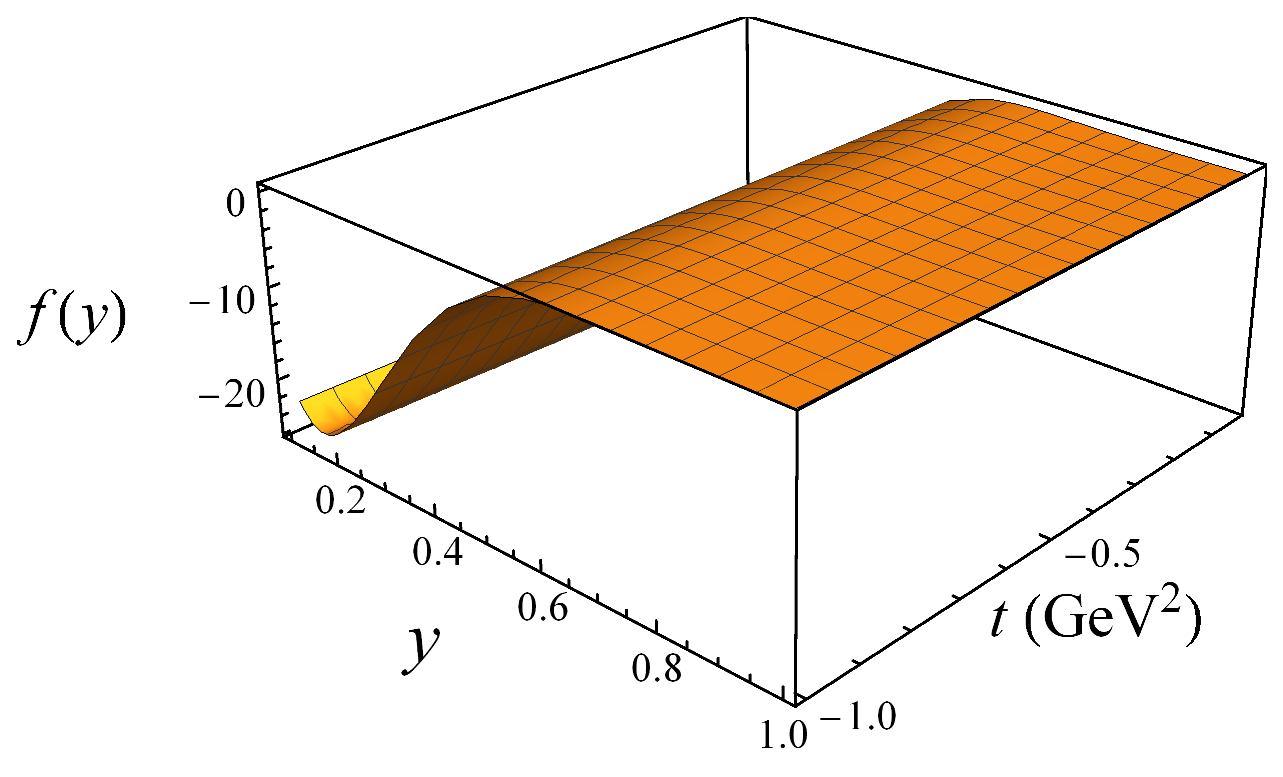
\includegraphics[scale=0.5]{pic/rbw-q0}

\caption{do not sum $s_{1}$}

\end{figure}

\begin{figure}
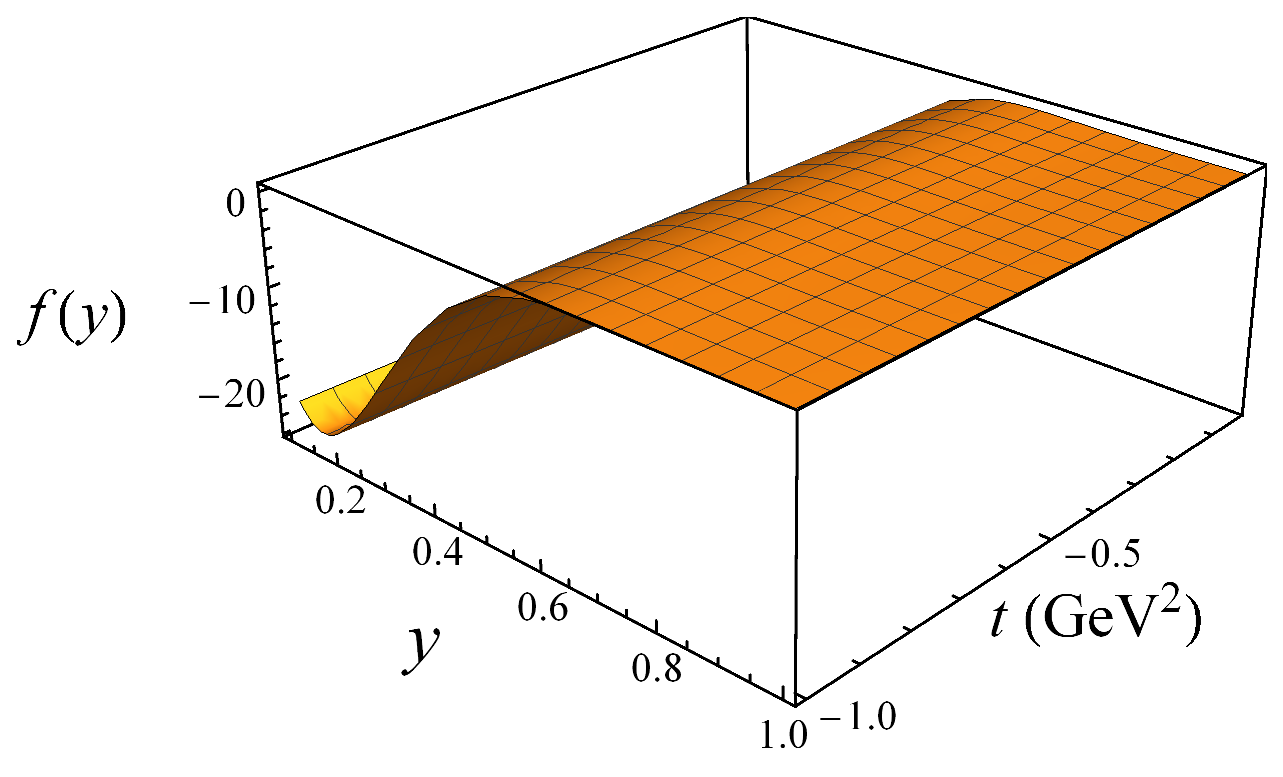
\includegraphics[scale=0.5]{pic/rbw-q0-spinsum}

\caption{sum $s_{1}$}
\end{figure}

\end{document}
